\chapter{Аналитическая часть}

В данном разделе будет проанализирована предметная область и выделены её основные сущности и ограничения значений их атрибутов.
Также будет выбран тип базы данных.

\section{Анализ предметной области}

Техническое задание к данной работе предполагает создание базы данных для погодного приложения.
Следовательно, необходимо проанализировать предметную область метеорологии для выделения сущностей и связей между ними, а также атрибутов данных сущностей.

\subsection{Актуальность проекта и рассмотрение аналогов}
Погодные приложения используются для доступа к метеорологическим прогнозам.
Предсказанием погоды занимаются специальные компании, которые лишь предоставляют данные о ней для конкретного региона.
Также существуют погодные сервисы, которые собирают погодные данные от этих компаний и предоставляют API, позволяющее приложениям получить эти данные для выбранного региона в виде JSON-файла~[19].
Чтобы конечный пользователь смог просмотреть прогноз погоды, разрабатываются специальные приложения.
С их помощью у пользователя есть возможность не только получить любую информацию о погоде с какого-либо сервиса, но и просмотреть её в удобном формате.
Часто планы человека подвержены влиянию погоды, следовательно, наличие такого приложения может быть полезным.

\subsection{Cущности в метеорологии}
Главной задачей метеорологии является прогнозирование погоды~[2].
Тогда основной сущностью исследуемой предметной области является погода.
Необходимо выяснить, какие атрибуты она имеет.
Погода определяется для какого-либо дня или часа, причём день представляется датой, состоящей из года, месяца и дня, а час -- номером от $1$ до $24$.
Таким образом, день и час являются атрибутами погоды.
Далее рассмотрены составляющие погоды, представляющие интерес для пользователей её прогнозов~[1]. 
Их список:
\begin{itemize}
    \item температура воздуха;
    \item атмосферное давление;
    \item скорость ветра;
    \item относительная влажность воздуха;
    \item видимость;
    \item облачность;
    \item осадки;
    \item гроза;
    \item туман;
    \item метель;
    \item пыльные бури;
    \item гололёд.
\end{itemize}
Ещё один часто выделяемый параметр погоды -- ощущаемая температура~[4]~[5].
Он нужен для субъективного понимания пользователем текущей погоды.
Перечисленные параметры, в зависимости от способа формализации, могут быть как числовыми, так и логическими, и являются атрибутами погоды.

Важной особенностью погоды является локальность.
Это значит, что она всегда ассоциируется с определённым географическим местом.
В сервисах, предоставляющих информацию о погоде, в качестве такого места рассматривается город~[4]~[5].
Причём город имеет ряд своих атрибутов, таких как:
\begin{itemize}
    \item название;
    \item страна;
    \item место на карте.
\end{itemize}
Более того, на один и тот же город могут ссылаться многие сущности погоды.
Поэтому его следует рассматривать как отдельную сущность предметной области.

Согласно предметной области, существует такое понятие, как прогноз погоды~[4].
Если погода определена для будущего времени, то она является прогнозом.
Поэтому нет смысла рассматривать прогноз как отдельную сущность.

Таким образом, к основным сущностям предметной области метеорологии относятся погода и город.

\subsection{Формализация сущностей предметной области}
В данном разделе будут формализованы сущности погоды и города.
Для формализации понятия погоды необходимо выделить набор формальных параметров погоды на основе выделенных её составляющих.
Для этого проанализированы существующие погодные сервисы: Яндекс Погода~[4], AccuWeather~[5], Погода <<Mail.ru>>~[6], The Weather Channel~[7].

Сначала рассмотрены атрибуты, которые можно описать простыми типами данных.
Такие параметры погоды, как температура, давление, влажность, скорость ветра и видимость являются числовыми и измеряются в градусах по Цельсию, миллиметрах ртутного столба, процентах, метрах в секунду и километрах соответственно.
Видимость характеризуется максимальным расстоянием, на котором среднестатистический человек может что-либо увидеть.
Погодные сервисы следят за двумя видами осадков: дождевыми и снежными и измеряют их в миллиметрах или сантиметрах.
Таким образом, осадки представляются двумя числами: количеством выпавшего дождя и снега в миллиметрах и сантиметрах соответственно.
Числовые атрибуты могут быть как целыми, так и вещественными.
Температура и видимость отнесены к вещественным числам, а остальные параметры -- к целым.

Далее рассмотрены параметры погоды, плохо поддающиеся численному описанию.
К ним относится облачность и наличие каких-либо природных явлений.
Облачность представляется либо процентом части неба над городом, закрытого облаками, либо перечислением: солнечно, облачно с прояснениями, пасмурно.
Природные явления всегда задаются перечислением~[4]~[7]: гроза, дождь, туман, солнце, снег и метель и другие.
Таким образом, удобно ввести тип погоды -- сущность, которая будет содержать следующую информацию о природных явлениях:
\begin{itemize}
    \item текстовое описание;
    \item иллюстрирующую картинку в виде массива байт;
    \item иллюстрирующую картинку в виде ссылки;
    \item целочисленный идентификатор типа.
\end{itemize}
Например, среди используемых типов могут быть: гроза, морось, дождь, ливень, туман, солнце, облачно с прояснениями, пасмурно, снег, метель.
Точный набор типов погоды может изменяться в зависимости от погодного сервиса, используемого приложением, поэтому с точки зрения базы данных не важно, какие именно природные явления будут выделены.
Таким образом, один из атрибутов погоды -- идентификатор её типа, что позволяет хранить информацию о нечисловых параметрах.
Но атрибут, характеризующий облачность, удобно рассматривать как отдельный числовой параметр, изменяющийся от $0$ до $100$ процентов, так как тогда его можно будет совмещать с любым типом погоды.

Необходимо также выделить точный набор параметров такой сущности города.
Он характеризуется названием, географическим расположением и названием страны.
Под географическим расположением подразумевается широта и долгота, выраженные в вещественных числах~[3].

Далее рассмотрены атрибуты погоды, относящиеся ко времени.
День описывается датой, которая содержит год, месяц и день, а час всегда привязан к определённому дню и указывается порядковым номером относительно его начала.
Возникает вопрос: в каком виде лучше представить данные временные параметры.
Если хранить дату в привычном для пользователя формате, то есть как строчку, то возникают следующие неудобства:
\begin{itemize}
    \item
        пользователи из разных стран используют разный формат даты и времени, что требует преобразование форматов друг к другу;
    \item
        если погода определена для какого-то дня в целом, то не очевидно, что следует хранить в качестве времени;
    \item
        сравнение дат, представленных в виде строки, производится дольше, чем сравнение чисел и требует специальных средств СУБД.
\end{itemize}
Другой вариант хранения даты -- количество секунд с начала эпохи, то есть с 1 января 1970 года.
Таким образом, дату, извлечённую из базы данных можно будет преобразовать к нужному формату, а сравнение дат сведётся к сравнению целых чисел.

У погоды есть одна важная особенность: если она определена для дня в целом, то она может содержать параметры, не актуальные для той погоды, которая определена для конкретного часа или текущего момента времени~[4]~[5]~[7].
А поскольку приложение и база данных, вероятнее всего, будут развиваться и дорабатываться, таких параметров может стать ещё больше.
Например, к ним относится номер часа, среднесуточная температура, время заката, фаза луны и т. д.
Поэтому удобно разделить погоду на две сущности: суточную погоду и почасовую.
Многие атрибуты данных сущностей будут одинаковы, но появится возможность дополнять их независимо друг от друга.
Точный набор параметров дневной и почасовой погоды будет определён на этапе проектирования базы данных исходя из возможностей, предоставляемых погодным сервисом.

В результате рассуждений в данном разделе, все сущности предметной области метеорологии выделены и формализованы.

\subsection{Граничные значения параметров сущностей}
После описания сущностей предметной области необходимо представить требования к их целостности.
Далее представлена таблица~\ref{table:weather_parameters}, содержащая ограничения на числовые параметры погоды и города.

\begin{table}[h!]
    \centering
    \begin{tabular}{ |c|c|c| }
        \hline
            \textbf{Параметр погоды} & \textbf{Ограничения} & \textbf{Единицы измерения} \\
        \hline
            температура & $-273$ -- $\infty$ & \textdegree C \\
        \hline
            ощущаемая температура & $-273$ -- $\infty$ & \textdegree C \\
        \hline
            скорость ветра & $0$ -- $\infty$ & м/с \\
        \hline
            давление & $0$ -- $\infty$ & мм рт. ст. \\
        \hline
            относительная влажность & $0$ -- $100$ & \% \\
        \hline
            дождевые осадки & $0$ -- $\infty$ & мм \\
        \hline
            снежные осадки & $0$ -- $\infty$ & cм \\
        \hline
             дата & $0$ -- $\infty$ & секунды \\
        \hline
            \textbf{Параметр города} & \textbf{Ограничения} & \textbf{Единицы измерения} \\
        \hline
            широта & $-90$ -- $90$ & градусы \\
        \hline
            долгота & $-180$ -- $180$ & градусы \\
        \hline
    \end{tabular}
    \caption{\centering Параметры погоды, их единицы измерения и граничные значения}
    \label{table:weather_parameters}
\end{table}

\section{Формализация задачи}
Разрабатываемое погодное приложение предполагает ровно $3$ роли пользователей в зависимости от их подписки.
Роль определяет набор функций, предоставляемых базой данных.
Далее на рисунке~\ref{fig:use-case} представлен полный список функций разрабатываемой базы данных, а также её ролевая модель.
Наличие той или иной роли может зависеть от подписки пользователя.

\begin{figure}[H]
	\centering
	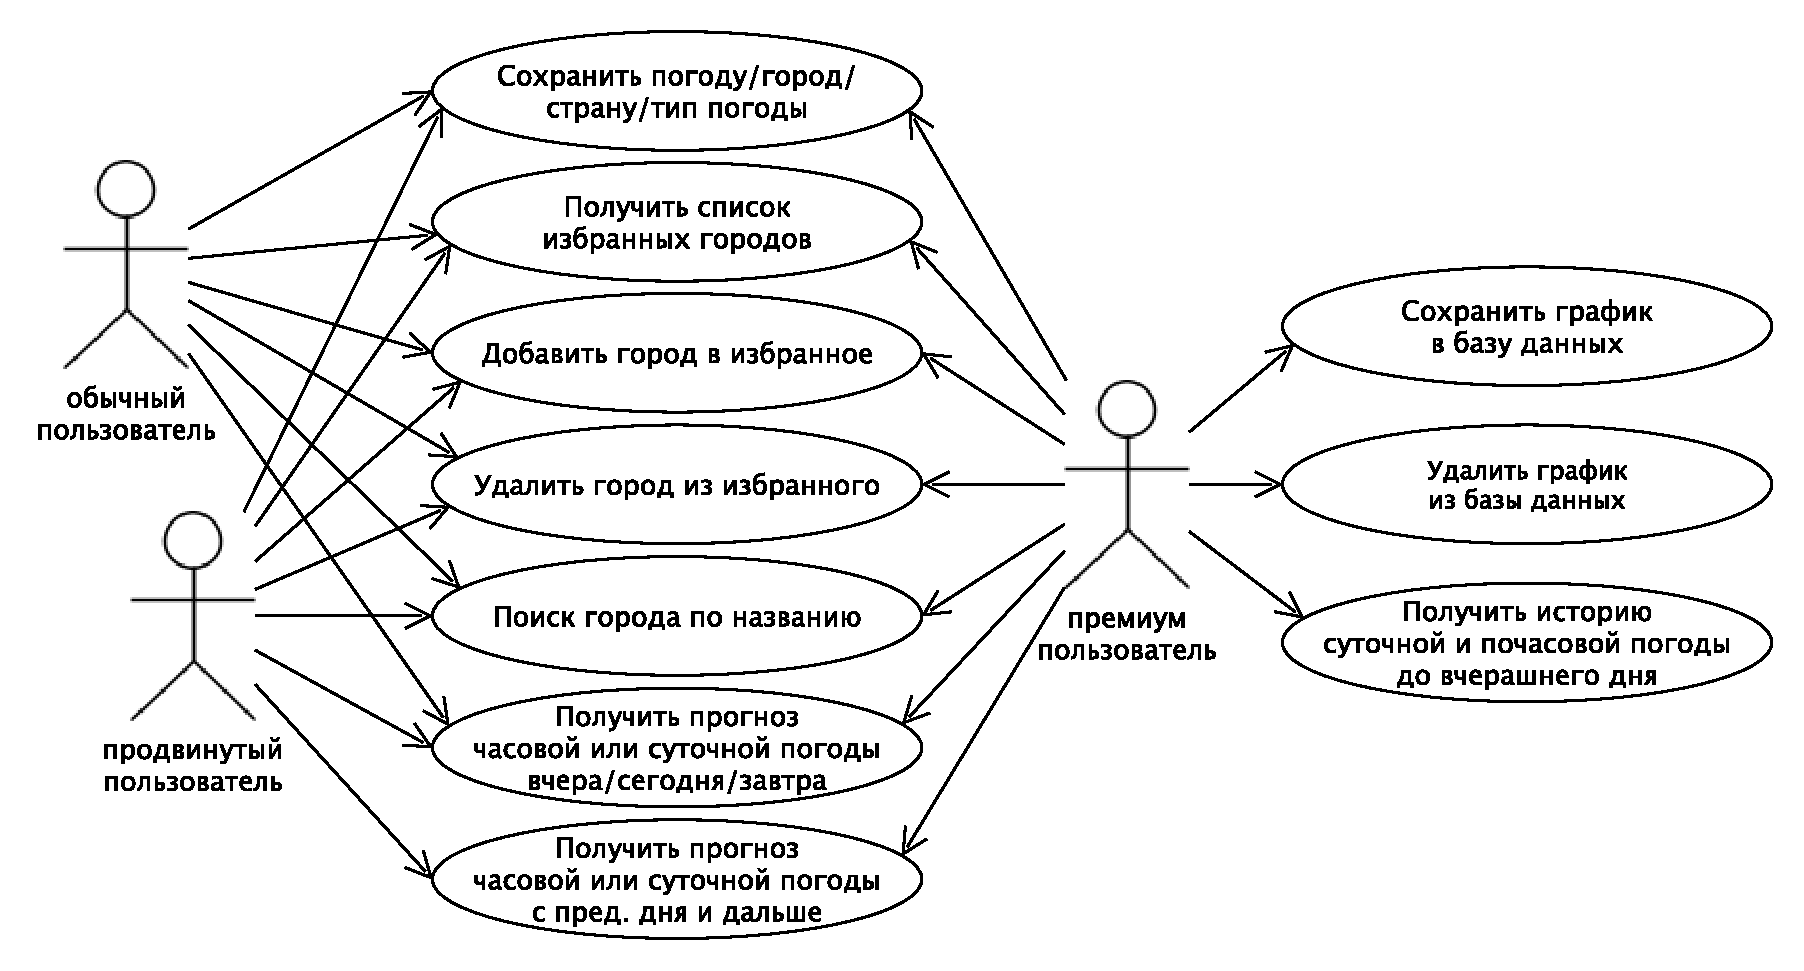
\includegraphics[width=\textwidth]{tools/img/db_usecase.pdf}
	\caption{
        Диаграмма прецедентов для разрабатываемой базы данных с учётом ролевой модели
    }
	\label{fig:use-case}
\end{figure}


\section{Требования к базе данных}
Для проектирования базы данных необходимо определить набор требований к ней.
Выделены следующие критерии для выбора типа базы данных:
\begin{itemize}
    \item наличие возможности обеспечить безопасность данных, то есть реализовать ролевую модель (К0);
    \item наличие возможности отслеживания целостности данных (К1);
    \item наличие возможности сжатия данных (К2);
    \item наличие возможности ускорения доступа к данным с помощью их индексации (К3);
    \item наличие возможности хранить отношения многие-ко-многим (К4);
    \item наличие возможности дешёвой разработки и сопровождения (К5);
    \item наличие возможности удалённого хранения части данных (К6).
\end{itemize}

Важным критерием (К5) является возможность не только простой разработки, но и недорогого сопровождения.
Необходимо формализовать данный критерий, так как он субъективен.
Цена разработки пропорциональна её времени, которое зависит от наличия документации для используемых технологий.
Также на цену влияет поддержка используемых технологий различными операционными системами, так как если приложение и базу данных нужно будет перенести на другую ОС, то может потребоваться использование других технологий, что затрудняет разработку.
Приведённые факторы формирования цены напрямую зависят от популярности технологий, используемых при создании программного обеспечения.
Таким образом, критерий <<К5>> можно формализовать как то, что используемый тип баз данных реализован в виде технологии, являющейся одной из самых популярных или поддерживающейся одной из самых больших IT-компаний.

Другим важным требованием (К6) является удалённое хранение сущностей пользователей.
Это обеспечит возможность авторизации на другом устройстве.

База данных должна предоставлять достаточно возможностей чтобы хранить все необходимые приложению сущности и связи между ними.
На рисунке~\ref{fig:er-chen} представлена диаграмма сущность-связь.
\begin{figure}[H]
	\centering
	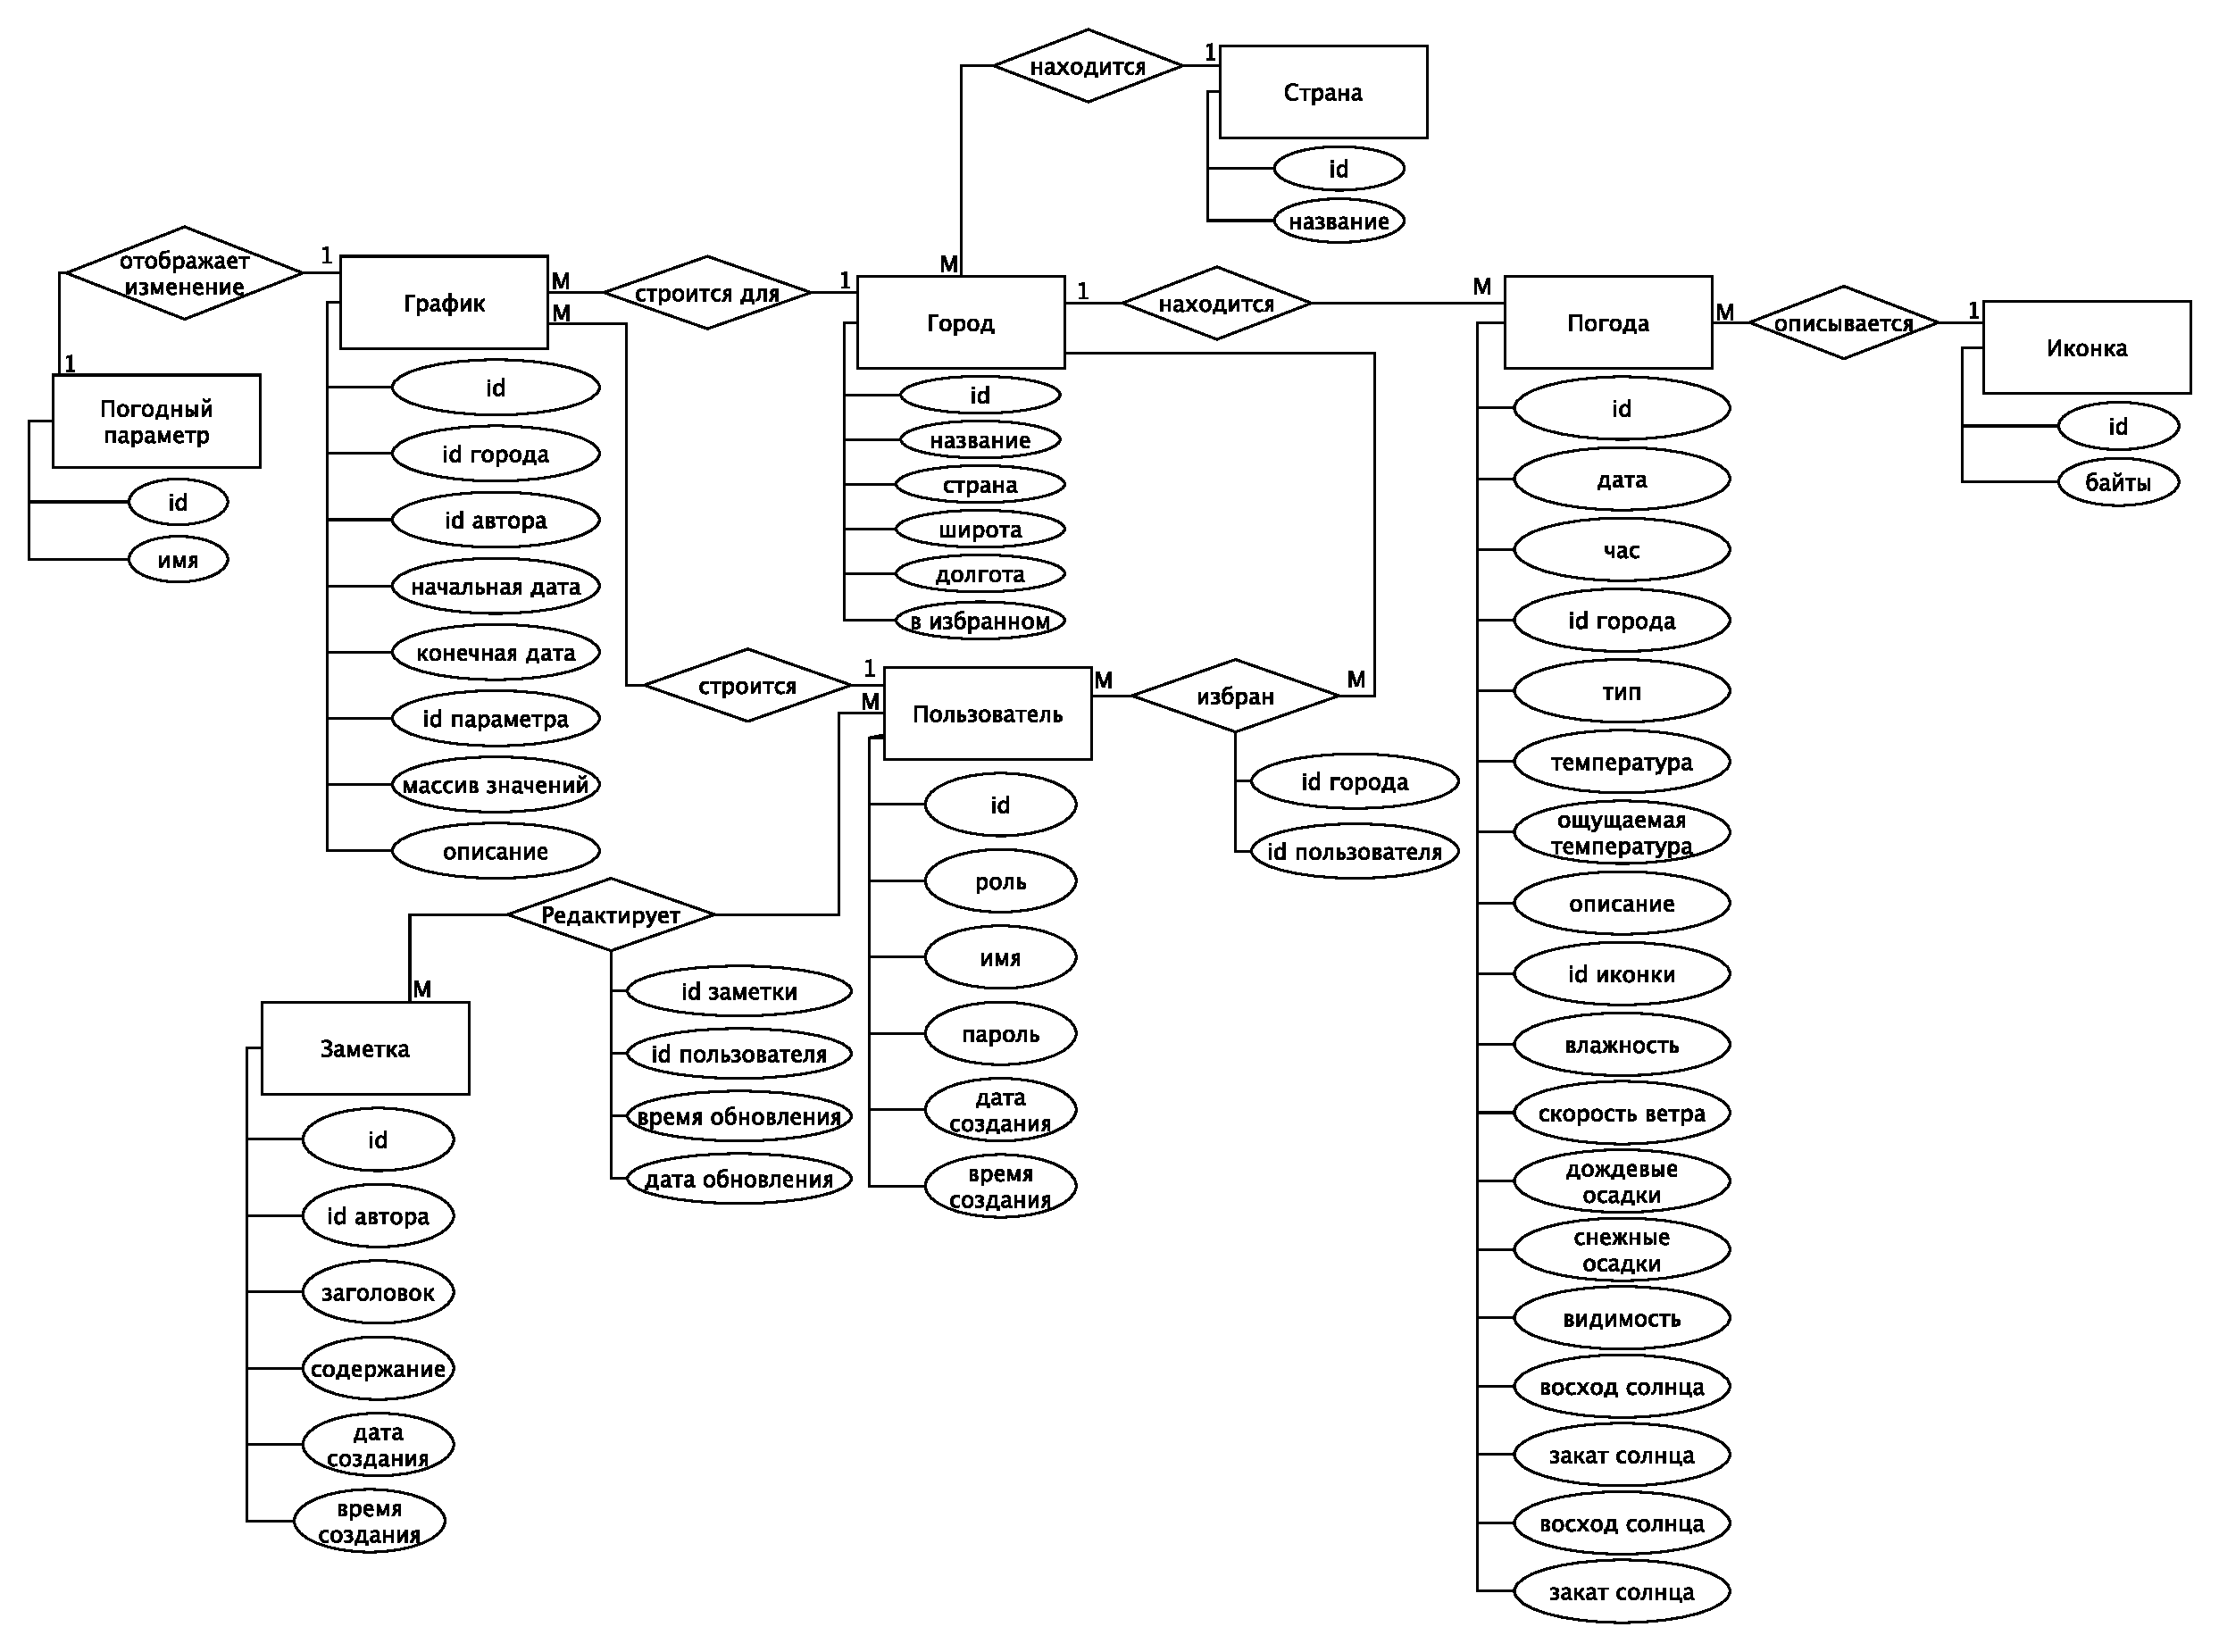
\includegraphics[width=\textwidth]{tools/img/er-chen.pdf}
	\caption{
        Диаграмма сущность-связь разрабатываемой базы данных в нотации Чена
    }
	\label{fig:er-chen}
\end{figure}

\section{Выбор типа базы данных}
Далее представлена таблица~\ref{table:cmp_model}, отображающая результаты сравнения моделей представления данных.
\begin{table}[h!]
    \centering
    \begin{tabular} { |c|c|c|c|c|c|c| }
        \hline
        \hspace{0pt} & \multicolumn{6}{|c|}{Критерий} \\
        \hline
        Тип базы данных & К0 & К1 & К2 & К3 & К4 & К5 \\
        \hline
        Реляционная & + & + & + & + & + & + \\
        \hline
        Документальная & + & - & - & + & + & + \\
        \hline
        Графовая & + & + & - & + & + & - \\
        \hline
        \end{tabular}
    \caption{\centering Сравнение типов баз данных, основанных на моделях представления}
    \label{table:cmp_model}
\end{table}
Существуют различные типы баз данных.
От типа зависит способ хранения информации и алгоритмы доступа к ней.
Каждый тип баз данных имеет некоторые особенности, которые могут иметь ключевое значение для удовлетворения выделенным требованиям.
Базы данных разделены на группы по модели представления данных и способу доступа к ним~[11].

К способам доступа к данным относятся~[11]:
\begin{itemize}
    \item клиент-серверный;
    \item файл-серверный;
    \item встраиваемый.
\end{itemize}

Одно из требований, предъявленных к базе данных -- удалённое хранение данных о пользователях (К6).
Это можно сделать с помощью клиент-серверной или файл-серверной модели взаимодействия.
Остальные сущности лучше хранить локально, так как нет необходимости публикации этих данных для совместного использования на нескольких устройствах.

К основным типам баз данных относительно модели представления информации относятся~[11]:
\begin{itemize}
    \item реляционные;
    \item документальные;
    \item графовые.
\end{itemize}

Реляционная база данных является самой популярной для решения практических задач~[8], а также, в отличие от остальных, поддерживает стандартный язык запросов -- SQL, который можно использовать на всех ОС.
Таким образом, реляционная база данных удовлетворяет критерию <<К5>>.
Документальные базы данных существуют на всех популярных ОС, таких как Android, IOS, Linux, Windows, macOS.
Также данный тип баз данных реализован в виде СУБД Firebase, поддерживаемой компанией Google~[14].
Поэтому документальные базы данных тоже удовлетворяют критерию <<К5>>.

В результате сравнения типов баз данных, определено, что целесообразно выбрать локальную реляционную СУБД и клиент-серверную документальную СУБД, что позволит выделить сущности, переносимые между устройствами.
К данным, хранимым удалённо, относятся сущности пользователей и наборы идентификаторов избранных ими городов.
Остальные данные следует хранить локально.

\section*{Выводы из аналитической части}
В данном разделе была проанализирована предметная область метеорологии, в результате чего определены её основные сущности, а также атрибуты погоды и их граничные значения.
Затем определены требования к разрабатываемой базе данных и проведён анализ существующих, в результате чего сделан выбор типа базы данных.
Таким образом, получены все необходимые сведения для проектирования.